\documentclass[]{article}
\usepackage[utf8]{inputenc}
\usepackage{pdfpages}
\usepackage{amsmath}
\usepackage{amssymb}
\usepackage{graphicx}
\usepackage{geometry}
\usepackage{enumitem}
\usepackage{amsthm}
\usepackage{stmaryrd}
\usepackage{mathtools}
\usepackage{mathrsfs}
\usepackage{bbm}

\geometry{hmargin=2cm}

% Environnement type théorème
\newtheorem{mythm}{Théorème}
\newtheorem{myproposition}{Proposition}
\newtheorem{myproperty}{Propriété}
\newtheorem{mylemma}{Lemme}
\newtheorem{mycoro}{Corollaire}

% Environnement type texte
\theoremstyle{remark}
\newtheorem{mynot}{Notation}
\newtheorem{myrem}{Remarque}
\newtheorem{myexer}{Exercice}
\newtheorem{myproof}{Preuve}
\newtheorem{myexmpl}{Exemple}

% Environnement de définition
\theoremstyle{definition}
\newtheorem{mydef}{Définition}
\newtheorem{myquestion}{Question}

\setlist[itemize]{label=-}

% Carré de fin de preuve
\newcommand{\cqfd}{
	\hfill$\square$
}

% Définition de fonction
\newcommand{\func}[5]{
#1 ~ : ~ \left\{ \begin{array}{lcl}
	#2 & \longrightarrow & #3 \\
	#4 & \longmapsto & #5
\end{array}
\right.
}

\newcommand{\fun}[3]{
#1 ~ : ~ #2 \longrightarrow #3
}

\newcommand{\funcinline}[5]{
	#1 \, : \, #2 \longrightarrow #3, ~ #4 \longmapsto #5
}

\newcommand{\funcshort}[3]{
	#1 \, : \, #2 \longrightarrow #3
}

\newcommand{\anonfunc}[4]{
	\left\{ \begin{array}{lcl}
		#1 & \longrightarrow & #2 \\
		#3 & \longmapsto & #4
	\end{array}
	\right.
}

\allowdisplaybreaks[4]

\newcommand{\vect}{\text{Vect}}

\newcommand{\card}{\text{Card }}

\newcommand{\DS}{\displaystyle}

\begin{document}
	\part{Analyse du signal}
	
	On munit à présent $L^2(\mathbb{R})$ du produit scalaire $\langle \cdot, \cdot \rangle$ défini par $$\langle f, g\rangle = \int_\mathbb{R} f(t) \overline{g(t)} dt$$
	et de la topologie induite par la norme correspondante.
	
	On remarquera qu'ici $L^2(\mathbb{R})$ désigne l'espace des fonctions de carré intégrable \textbf{quotienté par l'ensemble des fonctions nulles presque partout}. Ce passage au quotient est nécessaire pour que $\|\cdot \|_2$ soit une norme (au lieu d'une semi-norme).
	
	\section{Analyse multi-résolution}
	
	\subsection{Introduction}
	
	Nous allons enrichir la théorie des espaces de Hilbert d'une notion de "finesse"  particulièrement adaptée à l'objet central de ce rapport. En effet, dans le cadre de l'approximation d'un signal, que nous modélisons par une fonction $\mathbb{R}^n \rightarrow \mathbb{R}^m$, cette notion prend tout son sens comme le montre l'image ci-dessous.
	
	\begin{figure}[h]
		\centering
		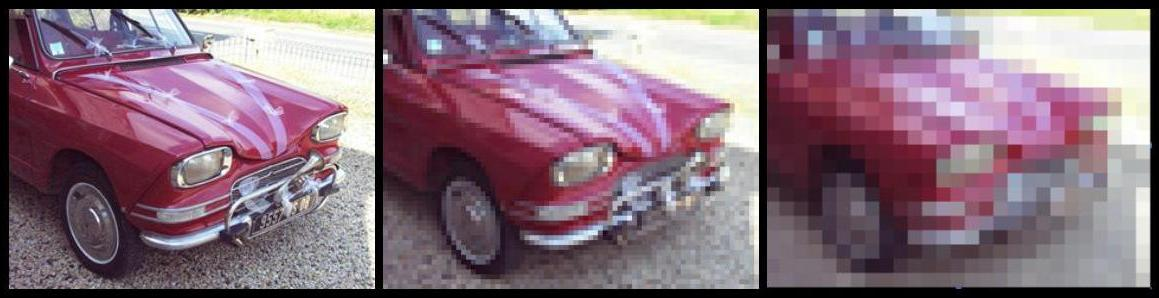
\includegraphics[width=350pt]{Resolution_wikipedia.jpg}
		\caption{Une image de voiture pour trois résolutions différentes}
	\end{figure}
	
	Les images peuvent être modélisées comme des fonctions de $\mathbb{R}^2$, pour les coordonnées spatiales, dans $\mathbb{R}$ (resp. $\mathbb{R}^3$) dans le cas d'une image en noir et blanc (resp. en couleur RVB). Dans le cas d'un signal sonore, sachant qu'un son est une onde, il peut être représenté par une fonction de $\mathbb{R}$, pour le temps, dans $\mathbb{R}$, pour l'amplitude de d'oscillation.
	
	Avant de définir l'analyse multi-résolution, explorons plus profondément cette notion de "finesse".
	
	\subsubsection*{Quelle finesse !}
	
	Nous allons prendre pour exemple les signaux unidimensionnels (tels les sons). Soit $\funcshort{f}{[0, 1[}{\mathbb{R}}$ une fonction continue, nous allons l'approximer par des fonctions constantes par morceaux (dites étagées), dont les morceaux sont de plus en plus petits.
	
	\begin{figure}[h]
		\label{sine-stairs}
		\centering
		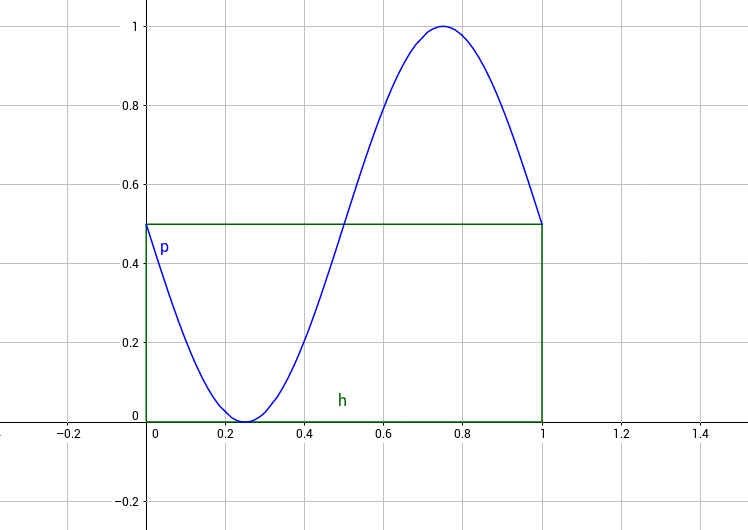
\includegraphics[width=150pt]{sin_1.png}
		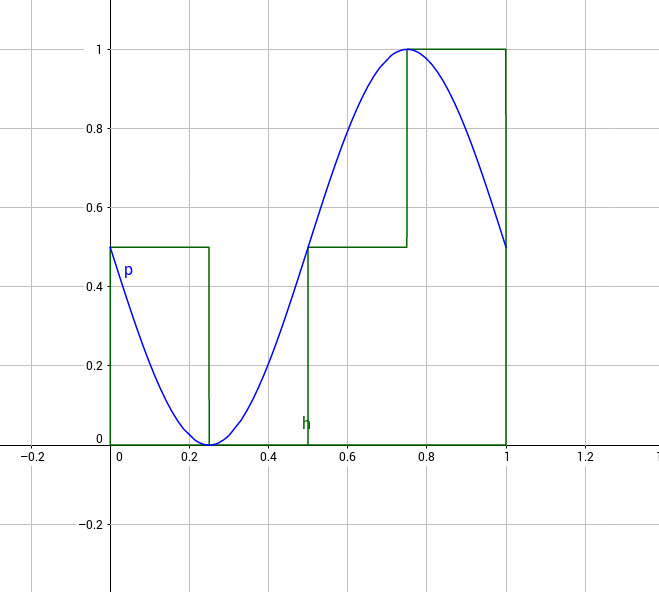
\includegraphics[width=150pt]{sin_2.png}
		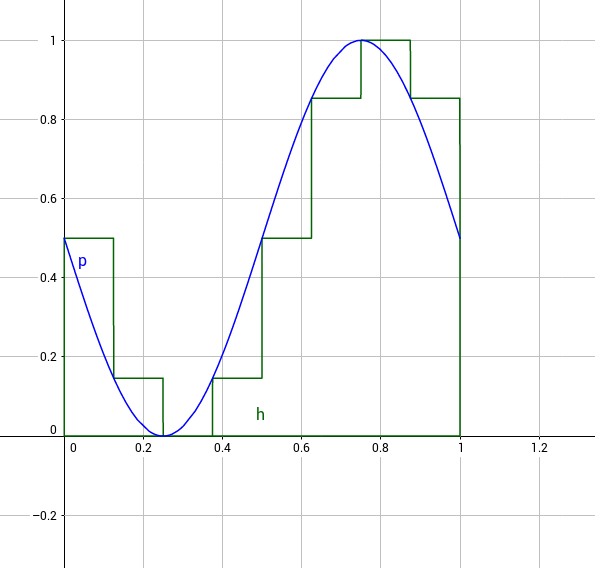
\includegraphics[width=150pt]{sin_4.png}
		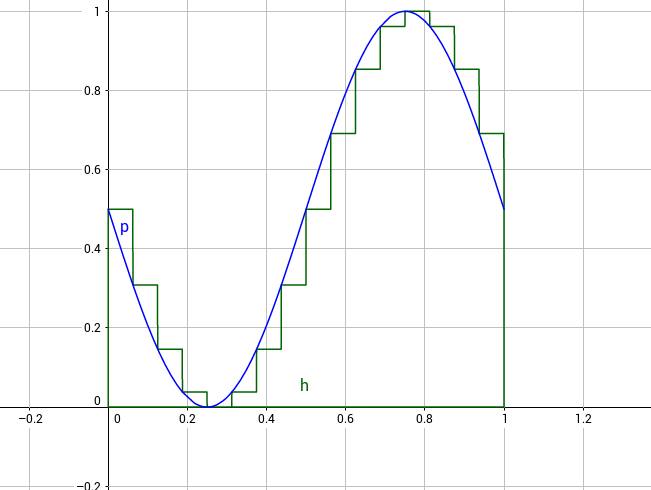
\includegraphics[width=150pt]{sin_8.png}
		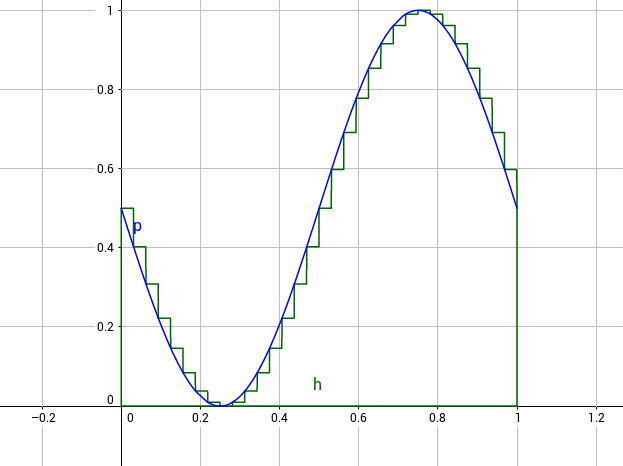
\includegraphics[width=150pt]{sin_16.png}
		\caption{$f$ approximée par des fonctions dont les morceaux sont de tailles 1, 1/2, 1/4, 1/8 et 1/16}
	\end{figure}
	
	\newpage
	
	Sur la figure on approxime $f$ par des fonctions $f_n$ étagées dont les morceaux sont de tailles $2^{-n}$, on peut voir chaque $f_n$ comme une combinaison linéaire de fonctions caractéristiques de la forme suivante $$f_n = \sum_{k = 0}^{2^n} a_{n, k} \mathbbm{1}_{[k 2^{-n}, (k+1)2^{-n}[}$$
	
	La première remarque que l'ont peut faire est que chaque $\mathbbm{1}_{[k 2^{-n}, (k+1)2^{-n}[}$ est le translaté de $\mathbbm{1}_{[0, 2^{-n}[}$, que l'on notera $I_n$. On réécrit alors $$f_n(x) = \sum_{k = 0}^{2^n} a_{n, k} I_n\left(x - k 2^{-n}\right)$$
	
	La seconde est que $I_n$ est une contraction de $I_1$ que l'on notera $I$. On en tire notre dernière réécriture :
	
	$$f_n(x) = \sum_{k = 0}^{2^n} a_{n, k} I \left(\frac{x - k 2^{-n}}{2^{-n}}\right) = \sum_{k = 0}^{2^n} a_{n, k} I \left(2^n x - k\right)$$
	
	Ainsi si on fixe $I = \mathbbm{1}_{[0, 1[}$ comme fonction de référence dans notre décomposition, la suite de fonctions $(f_n)_n$ est entièrement déterminée par les coefficients $(a_{n, k})_{n, k}$
	
	\subsection{L'analyse multi-résolution}
	
	Dans l'exemple introductif, pour tout $n$ on a pu voir que $f_n$ était une combinaison linéaire du translaté d'une fonction $I_n$, $f_n$ appartenait alors à l'espace vectoriel engendré par les translations de $I_n$. De plus, chaque $I_n$ était la contraction de la fonction $I$ donnée par $I_n(t) = I\left(t 2^n\right)$. Il s'agissait d'un exemple d'analyse multi-résolution dont voici la définition :
	
	\begin{mydef}
		Une \textit{analyse multi-résolution} de l'espace $L^2(\mathbb{R})$ des fonctions de carré Lebesgue-intégrables est une suite $V = \{V_n\}_{n \in \mathbb{Z}} \subset L^2(\mathbb{R})$ de sous-espaces fermés de $L^2(\mathbb{R})$ satisfaisant aux conditions suivantes :

		\begin{equation}
			\label{growth}
			\forall n \in \mathbb{Z}, ~ V_{n} \subset V_{n+1} \text{ (croissance)}
		\end{equation}
		\begin{equation}
			\label{self-similarity}
			\forall n \in \mathbb{Z}, \forall f \in L^2(\mathbb{R}), ~ f \in V_n \Longleftrightarrow t \mapsto f \left(2 t\right) \in V_{n+1} \text{(auto-similarité)}
		\end{equation}
		\begin{equation}
			\label{rb-mra}
			\text{Il existe $\varphi \in V_0$ telle que $\{t \mapsto \varphi(t + k)\}_{k \in \mathbb{Z}}$ forme une base orthonormée de $V_0$}
		\end{equation}
		\begin{equation}
			\label{density}
			\overline{\bigcup V} = L^2(\mathbb{R}) \text{(densité)}
		\end{equation}
		\begin{equation}
			\label{inter}
			\bigcap V = \{0\}
		\end{equation}
		
		$\varphi$ est appelée \textit{fonction d'échelle}.
	\end{mydef}
	
	On peut généraliser par récurrence la propriété \ref{self-similarity} de la façon suivante :
	\begin{equation}
		\forall n \in \mathbb{Z}, \forall f \in L^2(\mathbb{R}), ~ f \in V_0 \Longleftrightarrow t \mapsto f \left(2^n t\right) \in V_{n}
	\end{equation}

	Ce qui met en évidence que plus $n$ est grand, plus l'espace $V_n$ contient des fonctions fines (la fonction est contractée horizontalement). D'après les propriétés \ref{self-similarity} et \ref{rb-mra}, on peut déduire que toute fonction de $V_n$ est une combinaison linéaire de contraction (d'un facteur au plus $2^n$) et translation de $\varphi$.

	\begin{mydef}
		Une analyse multi-résolution est dite \textit{localisée} si $\varphi$ vérifie la condition suivante
		\begin{equation}
			\label{localized}
			\forall m \in \mathbb{N}, \int_\mathbb{R} (1+|t|)^m |\varphi(t)|^2 dt < + \infty
		\end{equation}
	\end{mydef}
	
	Cette propriété porte bien son nom, si $\varphi$ la vérifie alors $|\varphi|^2$ décroît bien plus vite que tout polynôme en $\pm \infty$, suffisamment pour être intégrable. C'est le cas par exemple des gaussiennes et des fonctions à support compact. Une telle fonction $\varphi$ a une masse concentrée près de 0, ce qui limitera les "interférences" de ses translations dans leurs combinaisons linéaires.
	
	\begin{figure}[h]
		\centering
		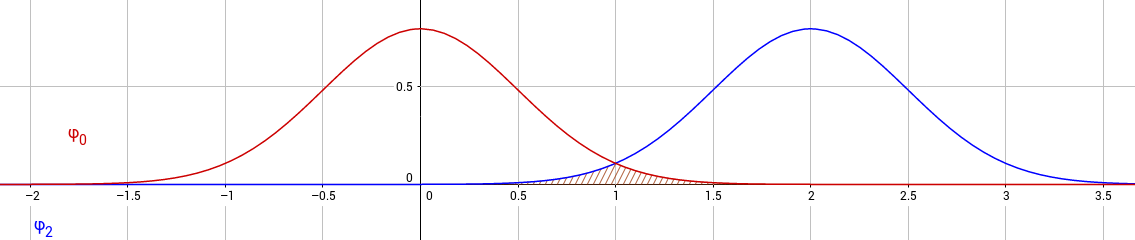
\includegraphics[width=450pt]{Localized.png}
		\caption{Les gaussiennes sont localisées}
	\end{figure}
	
%	\begin{myexmpl}
%		On reprend l'exemple précédent, avec $\varphi = \mathbbm{1}_{[0, 1[}$. On a alors pour tout $n, k \in \mathbb{Z}$ $$\varphi_{n, k} = 2^{n/2} \mathbbm{1}_{[k 2^{-n}, (k+1) 2^{-n}[}$$
%		
%		Pour tout entier $n$, la famille $\left(\varphi_{n, k}\right)_{k \in \mathbb{Z}}$ est effectivement une famille orthonormée : 
%		\begin{align*}
%			\langle \varphi_{n, k}, \varphi_{n, k'} \rangle &= \int_{\mathbb{R}} \varphi_{n, k} \varphi_{n', k'} d \lambda \\
%			&= \int_{\mathbb{R}} 2^{-n}  \mathbbm{1}_{[k 2^{-n}, (k+1) 2^{-n}[} \mathbbm{1}_{[k' 2^{-n}, (k'+1) 2^{-n}[} d \lambda \\
%			&= 2^{n}  \int_{\mathbb{R}} \mathbbm{1}_{[k 2^{-n}, (k+1) 2^{-n}[ \cap [k' 2^{-n}, (k'+1) 2^{-n}[} d\lambda \\
%			&= 2^{n} \lambda\left([k 2^{-n}, (k+1) 2^{-n}[ \cap [k' 2^{-n}, (k'+1) 2^{n}[\right)
%		\end{align*}
%		
%		On voit bien que les ensembles $[k 2^{-n}, (k+1) 2^{-n}[$ sont disjoints, donc la mesure de l'intersection considérée est soit nulle (si $k \neq k'$), soit égale à $\lambda([k 2^{-n}, (k+1) 2^{-n}[) = 2^{-n}$ (si $k = k'$).
%		
%		On retrouve bien $$\langle \varphi_{n, k}, \varphi_{n, k'} \rangle = \delta_{k, k'}$$
%		
%		On peut de plus approximer toute fonction de $L^2(\mathbb{R})$ aussi finement que souhaité par une fonction de $\DS \bigcup_{n \in \mathbb{Z}} V_n$.
%		
%		* Mq $V_n$ fermé
%		
%		* Mq toute fonction peut être approximé avec une finesse arbitraire par un élément de $\bigcup V$
%	\end{myexmpl}
		
	\newpage
		
	\subsection{Espace des détails}
	
	Pour tout $n$, on dénote par $\funcshort{P_n}{L^2(\mathbb{R})}{V_n}$ la projection orthogonale sur $V_n$ (on choisit les projections orthogonales car elles minimisent l'erreur commise en passant d'un espace à l'autre). Ainsi, pour tout $f \in L^2(\mathbb{R})$, $P_n (f)$ est l'approximation de $f$ avec une précision $2^{-n}$. Sur la figure $\ref{sine-stairs}$, on projette $f$ sur les espaces $V_0$ à $V_4$.
	
	Penchons nous sur ce qui se passe lorsqu'on passe d'une échelle plus fine à une échelle plus grossière.
	
	Soient $f \in L^2(\mathbb{R})$ et $f_n$ son approximation dans $V_n$ (c'est-à-dire $f_n = P_n(f)$). Le passage de $V_n$ à $V_{n-1}$ constitue une perte d'informations car on passe d'un espace plus fin à un espace plus grossier.
	
	\begin{align*}
		f_{n-1} &= P_{n-1} (f_n) \\
		&= P_{n-1}( (f_n - f_{n-1}) + f_{n-1}) \\
		&= \underbrace{P_{n-1} (f_n - f_{n-1})}_{0} + f_{n-1} \\
	\end{align*}
	
	La perte de précision, formalisée par $f_n - f_{n-1}$, est donc un élément du noyau de $P_{n-1}$, à savoir $V_{n-1}^\bot$. Mais $f_n - f_{n-1}$ étant dans $V_{n}$, l'ensemble regroupant les détails perdus en passant de $V_n$ à $V_{n-1}$ est $V_{n-1}^\bot \cap V_n$, c'est-à-dire le complémentaire orthogonal de $V_{n-1}$ dans $V_n$.
	
	\begin{mydef}
		Pour tout $n$ on définit \textit{l'espace de détails} $W_{n}$ comme le complémentaire orthogonal de $V_{n}$ dans $V_{n+1}$ $$V_{n+1} = W_n \stackrel{\perp}{\oplus} V_n$$
	\end{mydef}
	
	\paragraph*{}
	Les $(W_n)_n$ ne forment plus une famille monotone, mais leur somme recouvre tous les $V_n$. En d'autre termes, on peut à présent approximer toute fonction de $L^2(\mathbb{R})$ par une combinaison linéaire d'éléments de $\DS \bigoplus_{n \in \mathbb{Z}} W_n$.
	
	\begin{myproof}
		Soit $n_0 \in \mathbb{Z}$, on a par définition des $(W_{n})_n$
		
		\begin{align*}
			V_{n_0+1} &= V_{n_0} \oplus W_{n_0} \\
			&= V_{n_0 - 1} \oplus \left(W_{n_0 - 1} \oplus W_{n_0} \right) \\
			& \cdots \\
			&= V_{n_0 - N} \oplus \left(\bigoplus_{n = n_0 - N}^{n_0} W_n \right) \\
			& \cdots \\
			&= \bigcap V \oplus \left(\bigoplus_{n = - \infty}^{n_0} W_n \right) \\
			&= \{0\} \oplus \left(\bigoplus_{n = - \infty}^{n_0} W_n \right) \\
			&= \bigoplus_{n = - \infty}^{n_0} W_n
		\end{align*}
		
		On en déduit ainsi $\DS \bigcup V = \bigoplus_{n \in \mathbb{Z}} W_n$ en faisant tendre $n_0$ vers $\infty$ (ou plutôt en faisant l'union à gauche et à droite pour tout $n_0 \in \mathbb{Z}$).
		
		\cqfd
	\end{myproof}
	
	Comme on l'a dit, les $(W_n)_n$ ne forment pas une suite d'espaces emboîtés (ils sont même orthogonaux deux à deux), cependant ils vérifient encore les conditions d'auto-similarité et de stabilité par translation.

	\begin{mydef}
		Il existe une fonction normée $\psi$ - appelée \textit{ondelette} - engendrant $W_0$ par translation et de moyenne nulle (d'intégrale nulle).
		
		On admettra son existence \footnote{Voir \textit{Wavelets and Multiscale Signal Processing} d'Albert Cohen pour une démonstration de l'existence.}, mais elle peut être construite explicitement à partir de $\varphi$.
	\end{mydef}
		
	On définit encore une fois la famille $\Psi = \{\psi_{n, k}\}_{n, k \in \mathbb{Z}}$ par $\psi_{n, k}(t) = 2^{-n/2} \psi(2^{n} t - k)$, et cette fois ci ... cette famille est une base orthonormée de $\DS \bigoplus_{n \in \mathbb{Z}} W_n$ ! Et donc une base hilbertienne de $L^2(\mathbb{R})$ !
	
	Le fait que la famille soit normée est évident, le fait qu'elle soit orthogonale découle de l'orthogonalité des $W_n$.
	
	\begin{myexmpl}
		On prend comme exemple l'ondelette de Haar qui est donnée par $$\psi(t) = \left\{
		\begin{array}{cl}
			0 & x < 0 \\
			1 & 0 \leqslant x < \frac{1}{2} \\
			-1 & \frac{1}{2} \leqslant x < 1 \\
			0 & 0 \leqslant x
		\end{array}
		\right.$$
	\end{myexmpl}
	
	\begin{figure}[h]
		\label{Haar}
		\centering
		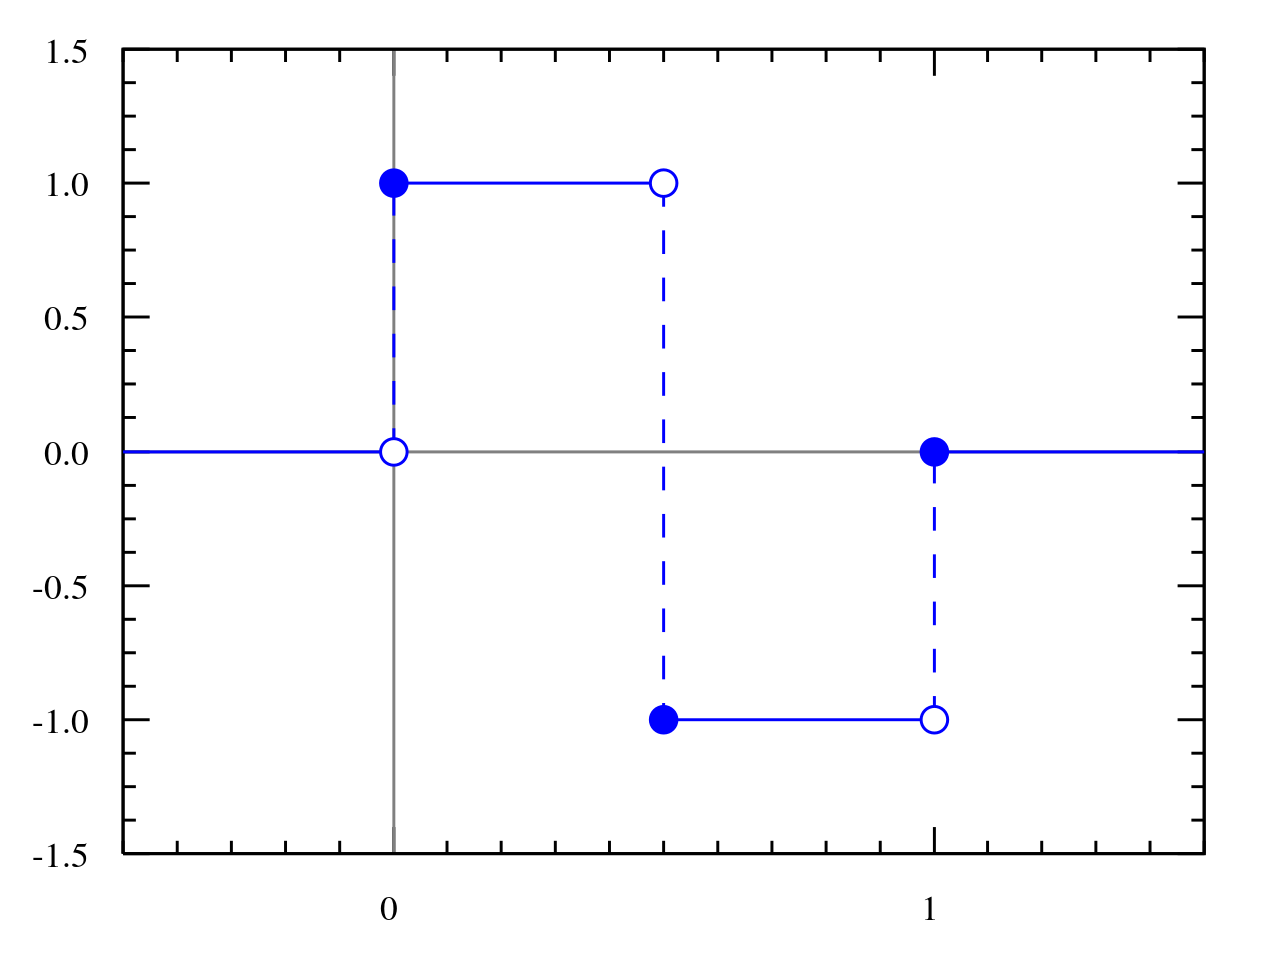
\includegraphics[width=150pt]{Haar.png}
		\caption{L'ondelette de Haar}
	\end{figure}
	
	$\psi$ est effectivement de moyenne nulle et $\Psi$ est orthonormée :
	
	\begin{align*}
		\langle \psi_{n, k}, \psi_{m, l}\rangle &= \int_{-\infty}^{\infty} \psi_{n, k}(t), \psi_{m, l}(t) dt \\
		&= 2^{\frac{m+n}{2}} \int_{-\infty}^{\infty} \underbrace{\psi(2^nt - k) \psi(2^mt - l)}_{h(t)} dt
	\end{align*}
	
	Si le graphe de la fonction $h$ admet un centre de symétrie sur $\mathbb{R}$ alors elle sera d'intégrale nulle (généralisation du fait que l'intégrale d'une fonction impaire est nulle). Cette remarque nous fournit un argument géométrique pour justifier que $\langle \psi_{n, k}, \psi_{m, l}\rangle$ vaut 1 si $n = m$ et $k = l$, et 0 sinon.
	
	Supposons $n \neq m$, alors les fonctions peuvent se positionner l'une par rapport à l'autre de quatre façons différentes, leur produit aura bien un centre de symétrie comme sur le figure.
		
	\begin{figure}[h]
		\centering
		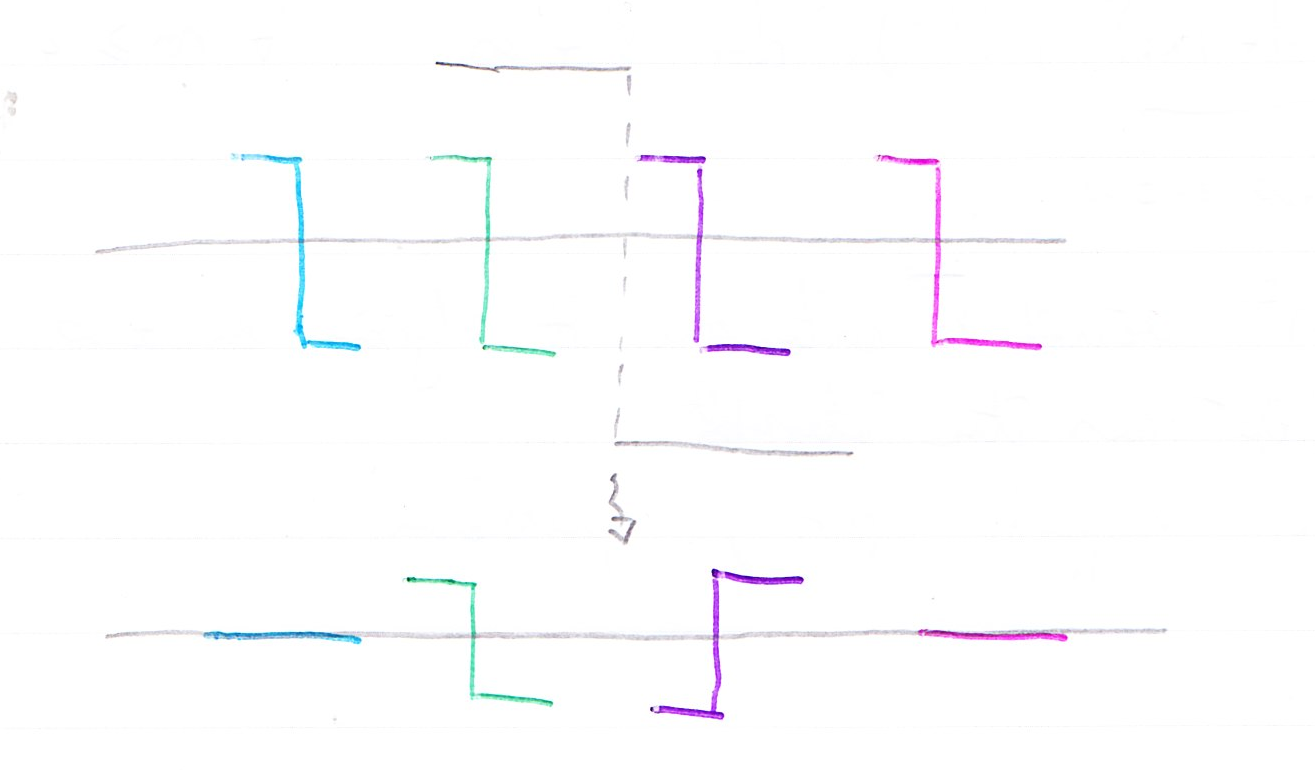
\includegraphics[width=350pt]{Haar_exemple.png}
		\caption{Le produit de deux ondelettes de Haar différentes  (la grise par une en couleur) possèdent un centre de symétrie dans $\mathbb{R}$.}
	\end{figure}
	
\end{document}